\documentclass[12pt]{article}
\usepackage{xr-hyper}
\externaldocument{supplement}
\usepackage{hyperref}
\usepackage[english]{babel}
\usepackage{graphicx}
\usepackage{framed}
\usepackage[normalem]{ulem}
\usepackage{amsmath}
\usepackage{amsthm}
\usepackage{amssymb}
\usepackage{amsfonts}
\usepackage{enumerate}
\usepackage{graphicx} % Allows including image
\usepackage{mathtools}
\hypersetup{
  linkcolor  = blue,
  citecolor  = blue,
  urlcolor   = blue,
  colorlinks = true,
} % color setup
\usepackage[utf8]{inputenc}
\usepackage[margin=1in]{geometry}
\usepackage{float} % for "H" placement specifier
\usepackage[authoryear]{natbib}
\usepackage{indentfirst}
\usepackage[dvipsnames]{xcolor}
\usepackage{array}
\usepackage{subcaption}
\usepackage{caption}
\usepackage[T1]{fontenc}
\usepackage{tikz}
\newcommand{\fatterdot}{\raisebox{0.15ex}{\tikz\filldraw[black,x=1.5pt,y=1.5pt] (0,0) circle (1);}}
\newcommand{\xn}{x^{\frac{1}{n}}}
\newcommand{\xnone}{x^{\frac{1}{n+1}}}

\newcommand{\R}{\mathbb{R}}
\DeclareUnicodeCharacter{FB01}{fi}
\DeclareUnicodeCharacter{FF0C}{,}
\DeclareMathOperator*{\Prob}{P}
\DeclareMathOperator*{\argmax}{arg\,max}
\DeclareMathOperator*{\argmin}{arg\,min}
\setlength\extrarowheight{1pt}

\newcommand\red[1]{{\color{red}#1}}

\bibliographystyle{plainnat}

\newtheorem{theorem}{Theorem}[section]
\newtheorem{corollary}{Corollary}[theorem]
\newtheorem{lemma}[theorem]{Lemma}
\newtheorem{prop}[theorem]{Proposition}
\newtheorem{defn}[theorem]{Definition}
\allowdisplaybreaks

\title{Recursive Full House Methodology}
\author{Daniel J. Eck$^1$, Shen Yan$^1$\thanks{Daniel J. Eck (\url{dje13@illinois.edu}); email addresses: Shen Yan (\url{shenyan3@illinois.edu})}}

\date{}

\begin{document}

\maketitle

{\centering
1. Department of Statistics, University of Illinois Urbana-Champaign \\}


\begin{abstract}

\end{abstract}

\section{Introduction}




\section{Model Setting}
\label{sec:modelsetting}
\textbf{This is taken directly from the paradox probability paper}: \\

We now motivate the structure of the Full House Model.  Let $N_i$ denote the size of population $i$. We distinguish between a \emph{population}, consisting of all individuals $N_i$ in context $i$, and a \emph{system}, which denotes the subset of individuals whose outcomes are observed or recorded. The system is determined by a selection mechanism that maps the full population into an observed sample of size $n_i$. We suppose that every individual $k = 1,\ldots, N_i$ has an underlying latent $\R$-valued aptitude $X_{i,1}, \ldots, X_{i,N_i} \overset{iid}{\sim} F_{X}$. Let $\textbf{X}_{i,-j}$ be the vector of all latent aptitudes not including the component $j$. We formalize the selection mechanism through an indicator function $S_{i,j} = 1_{i}\left(X_{i,j},\textbf{X}_{i,-j}\right)$, where $S_{i,j} = 1$ indicates inclusion in the observed system and a value of $S_{i,j} = 0$ indicates exclusion. This function may depend on the individual's aptitude relative to others in the population.

We now suppose that an individual $j$ included in system $i$ has an observed $\R$-valued statistic $Y_{i,j} \overset{iid}{\sim} F_{Y_i}$, $j = 1,\ldots,n_i$, with $n_i \leq N_i$. Under Full House Modeling, the observed values $Y_{i,j}$ are assumed to preserve the ranking induced by the latent aptitudes among the selected individuals.

Let $X_{i,(j)}$ and $Y_{i,(j)}$ denote the $j$th order statistic for system $i$. Here, larger values correspond to higher aptitude or achievement, so that $X_{i,(j)} > X_{i,(k)}$ whenever $j>k$. We form $(Y,X)$ pairs of random variables for each individual included in the system. These pairs are of the form $(Y_{i,(j)}, X_{i,(r_{i,j})})$, where $r_{i,j}$ indexes the rank of that individual's latent aptitude within the full population of size $N_i$.

As an example, consider the selection rule $S_{i,j} = 1 \;\Longleftrightarrow\; X_{i,j} \ge X_{i,(N_i-n_i+1)}$, which selects the top $n_i$ individuals in population $i$. In this case, the pairs take the form $(Y_{i,(j)}, X_{i,(N_i - n_i + j)})$ for $j = 1,\ldots,n_i$.

The key feature of Full House Modeling is the explicit connection between the elements forming the $(Y_{i,(j)}, X_{i,(r_{i,j})})$ pairs. This construction can be understood as a rank-preserving transformation between latent aptitude and observed achievement. Based on the probability integral transformation, Full House Modeling specifies this connection as
\begin{equation} \label{eq:truepar}
\begin{split}
  Y_{i, (j)} &= F_{Y_{i, (j)}}^{-1} \circ F_{X_{i, (r_{i,j})}} \left(X_{i, (r_{i,j})}\right), \\
  X_{i, (r_{i,j})} &= F_{X_{i, (r_{i,j})}}^{-1} \circ F_{Y_{i,(j)}} \left(Y_{i,(j)} \right),
\end{split}
\end{equation}
where $S_{i,j} = 1$, and both $F_{Y_i}$ and $F_X$ are continuous and invertible. We summarize Full House Modeling in the following definition.

\begin{defn} [Full House Model]
\label{def:fhm}
Consider populations indexed by $i$ with sizes $N_i$ and system sizes $n_i$, where $N_i \geq n_i$. Let latent variables $X_{i,j} \overset{iid}{\sim} F_X$, $j = 1,\ldots,N_i$, and define the selection indicators $S_{i,j} := 1_i(X_{i,j}, \mathbf{X}_{i,-j})$, where $S_{i,j}=1$ indicates inclusion in the observed system. Let $Y_{i,j} \overset{iid}{\sim} F_{Y_i}$, $j = 1,\ldots,n_i$, denote observed outcomes for the selected individuals. Form pairs $(Y_{i,(j)}, X_{i,(r_{i,j})})$, $j = 1,\ldots,n_i$, corresponding to the individuals for which $S_{i,j}=1$. Then the Full House Model generates $Y_{i,(j)}$ values according to \eqref{eq:truepar}, where $F_{Y_i}$ and $F_X$ are continuous and invertible.
\end{defn}

The Full House Model defines a joint distribution over $(X,Y)$ together with selection indicators $S_{i,j}$. Latent variables $X$ are drawn i.i.d.\ from $F_X$, and the selection indicators $S_{i,j}$ determine inclusion in the observed system. Conditional on inclusion, observed outcomes $Y$ are generated via a rank-preserving monotone coupling with $X$. In particular, the dependence between $X$ and $Y$ is induced through a quantile-matching transformation of their order statistics, ensuring that higher latent aptitude corresponds to higher observed achievement within each system. The stochasticity in the Full House Model arises entirely from the latent population $X$, while both selection and observed outcomes are deterministic functionals of $X$.

The Full House Model induces structural missingness by construction: for any individual $j$ such that $S_{i,j} = 0$, the corresponding observed statistic $Y_{i,j}$ is undefined. In subsequent sections, we consider probabilities involving both latent and observed quantities. To formalize this setting, we treat $Y_{i,j}$ as a random variable defined only on the event $\{S_{i,j}=1\}$. For example, $\Prob\big(X_{i,j}\in A,\; Y_{i,j}\in B,\; S_{i,j} = 1\big)$ is well-defined for Borel sets \(A,B\subset \mathbb R\), whereas $Y_{i,j}$ is not defined on $\{S_{i,j} = 0\}$. This perspective allows selection mechanisms to be incorporated into probabilistic statements without imputing counterfactual outcomes.

Definition~\ref{def:fhm} assumes a common latent aptitude distribution $F_X$ across contexts, while allowing the observed achievement distributions $F_{Y_i}$ to vary by system. This reflects a modeling choice in which the process generating latent aptitude is taken to be context-neutral, whereas the expression and measurement of aptitude may differ across contexts.


Direct evaluation of the order-statistic distributions in \eqref{eq:truepar} is often cumbersome. However, under continuity, they admit a convenient representation in terms of Beta distributions. In particular,
\begin{equation} \label{eq:betarepX}
F_{X_{i,(r_{i,j})}}\!\left(X_{i,(r_{i,j})}\right)
= F_{U_{i,(r_{i,j})}} \circ F_X\!\left(X_{i,(r_{i,j})}\right),
\quad U_{i,(r_{i,j})} \sim \mathrm{Beta}\!\left(r_{i,j},\, N_i - r_{i,j} + 1\right),
\end{equation}
and similarly,
\begin{equation} \label{eq:betarepY}
F_{Y_{i,(j)}}\!\left(Y_{i,(j)}\right)
= F_{U_{i,(j)}} \circ F_{Y_i}\!\left(Y_{i,(j)}\right),
\quad U_{i,(j)} \sim \mathrm{Beta}\!\left(j,\, n_i - j + 1\right).
\end{equation}
This representation allows \eqref{eq:truepar} to be computed via $F_X$, $F_{Y_i}$, and known Beta distributions, bypassing explicit order-statistic calculations. It also implies that latent aptitude can be recovered up to a monotone transformation without explicit knowledge of $F_X$.

Combining \eqref{eq:betarepX} and \eqref{eq:betarepY} yields
$$
X_{i,(r_{i,j})} = F_X^{-1}\!\left(
F_{U_{i,(r_{i,j})}} \circ F_{U_{i,(j)}} \circ F_{Y_i}\!\left(Y_{i,(j)}\right)
\right).
$$
Define $W_{i,j} = F_{U_{i,(r_{i,j})}} \circ F_{U_{i,(j)}} \circ F_{Y_i}(Y_{i,(j)})$. Since $F_X$ is monotone, so is its inverse, which implies
$$
W_{i_1,j_1} \ge W_{i_2,j_2} \;\;\Longrightarrow\;\; 
F_X^{-1}(W_{i_1,j_1}) \ge F_X^{-1}(W_{i_2,j_2}).
$$
Thus the ordering of latent aptitudes is invariant to $F_X$, and $F_X$ acts as a structural nuisance parameter for comparative analysis. In practice, Full House Modeling can therefore be implemented via observed-to-rank mappings without requiring explicit specification of the latent distribution.


\section{Recursive Full House Models}
\label{sec:rFHMsetup}

In this section we will investigate a simple extension to Full House Modeling in which Full House Models are repeatedly applied to individuals as they progress through iterations of some generic process. The general setup is that, in the first round, latent aptitude $X_{j} \overset{iid}{\sim} F_X$, $j = 1,\ldots,N$ will be generated  and then a label will be randomly assigned to each individual. There will be $m$ labels and each label will designate the outcome distribution. $F_{Y_{i,j}}$, $i = 1,\ldots,n$, $j = 1,\ldots,n_i$. Then outcomes will be realized as
\begin{equation} \label{eq:iteration}
  Y_{i,(r_{i,(j)})} = F_{Y_{i,j}}^{-1} \circ I_{r_{i,(j)},n_i-r_{i,(j)}+1}^{-1} \circ I_{j,N-j+1} \circ  F_X (X_{(j)}),	
\end{equation}
where $r_{i,(j)}$ is the rank of $X_{(j)}$ among the $n_i$ latent aptitudes also assigned label $i$. 

In the next iteration, all observations will be combined and then sorted in descending order by $Y_{i,(j)}$. The labels will be assigned in descending order, the largest $n_m$ values of $Y_{i,(j)}$ are assigned label $m$, the next largest $n_{m-1}$ values of $Y_{i,(j)}$ are assigned label $m-1$, and so on. We will setup these simulations so that $Y_i$ stochastically dominates $Y_{j}$ whenever $i > j$ so that higher outcomes are associated with higher labels. Then new $Y$ values are generated according to \eqref{eq:iteration}. The process will repeat until a pre-assigned stopping rule is satisfied. Note that this simulation setup assumes an immutable latent aptitude.


\subsubsection{Stop when highest latent aptitude is among the highest-performing group}
\label{sec:rFHMbestgroup}

Here we consider a recursive Full House Modeling setup described in Section~\ref{sec:rFHMsetup} in which the recursion stops at the first iteration when $X_{(N)}$ is assigned label $m$. Here we specify that $N = 100,000$, $m=200$, $n_i = 500$, $i = 1,\ldots,m$. We will assume that $X_j \overset{iid}{\sim} \text{Pareto}(1.16)$, $j = 1,\ldots,N$. And we will assume that $Y_{i,j} \overset{iid}{\sim} N(\mu_i,\sigma_i)$, $j = 1,\ldots,n_i$ and $i = 1,\ldots,m$. We will specify that the $\mu_i$s as a set of 200 equally spaced values between 60 and 80 with $\mu_i$ increasing in $i$, ie $\mu_i = 60 - 20/199 + 20i/199$, $i=1,\ldots,m$. %These values will be assigned to the index $i$ in increasing order, meaning that $\mu_1$ will be the smallest value $(60)$ and $\mu_m$ will be the largest value $(80)$. 
We will fix $\sigma_i = \sigma$ and consider $\sigma \in \{0.5,1,2\}$. These simulations will be repeated 500 times.

To illustrate the procedure, consider a simplified scenario in which all $X_{(j)}$ values are realized at their median value. With this simplification, $Y_{i,(r_{i,(j)})}$ in \eqref{eq:iteration} is approximately $F_{Y_{i,j}}^{-1}( (r_{i,(j)} - 1/3)/(n_i + 1/3))$ \citep{kerman2011closed}. And we have that $Y_{i,(n_{i})} - Y_{i+1,(n_{i+1}-1)} > \mu_{i+1} - \mu_{i}$ for all considered values of $\sigma$. The individual with latent ability $X_{(N)}$ will consistently attain the value $Y_{i,(n_{i})}$, regardless of their assigned group. Consequently, this individual's position among the $m$ groups will improve as the simulation advances. 

Results can be seen in Figure~\ref{Fig:rFHMrounds}. These Monte Carlo simulations reveal that it typically takes several rounds before the individual with the top aptitude belongs to the group that allows for the highest performances. On average, with $\sigma$ set to 0.5, 1, and 2, it takes 2.61, 4.19, and 7.46 rounds, respectively, for the individual with the top aptitude to join the highest-performing group (respective standard errors: 0.05, 0.09, 0.18). Deriving the distribution of this hitting time analytically under explicit FHM assumptions, and characterizing how it depends on $\sigma$ and grouping structure, remains an open problem. 

\begin{figure}[t!]
\begin{center}
	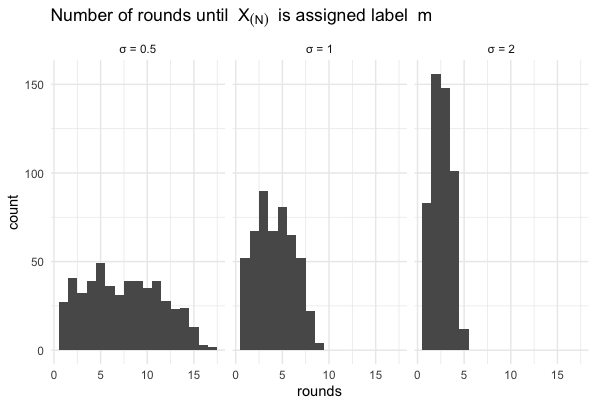
\includegraphics[scale=0.60]{rFHMrounds.png}
\end{center}	
\caption{The number of rounds that it takes for $X_{(N)}$ to be assigned label $m$ in a recursive Full House Modeling framework in Section~\ref{sec:rFHMsetup} with specifications in Section~\ref{sec:rFHMbestgroup}.}
\label{Fig:rFHMrounds}
\end{figure}

While the setting is stylized and assumes fixed latent aptitude, it illustrates how structural features of evaluative systems, not just randomness, can delay recognition of true potential. Whereas the paradox probability quantifies cross-sectional reversal risk, recursive Full House Modeling captures temporal persistence: the hitting time measures how many rounds elapse before latent aptitude and observed achievement align. These findings resonate with a growing empirical literature on bias and distortion in algorithmic and educational evaluation systems, which we discuss further in the Discussion.





\section{Discussion}

Beyond baseball, the recursive Full House Modeling example in Section~\ref{sec:rFHMbestgroup} speaks to broader concerns in educational evaluation and admissions. When students transition across institutions of varying selectivity, from less selective undergraduate programs to more selective graduate programs, or vice versa, observed performance metrics may systematically misrepresent underlying aptitude due to differences in both competition depth and measurement environments. The framework developed here provides a principled way to quantify such distortions, though substantial work remains to characterize the specific selection mechanisms and measurement properties that govern real educational pipelines. Our hope is that this methodology can eventually inform more equitable evaluation practices across educational and professional contexts where cross-institutional comparisons are routine but poorly understood.


\bibliography{FHM.bib}
\bibliographystyle{plainnat}


\end{document}


